\documentclass[]{article}
\usepackage{lmodern}
\usepackage{amssymb,amsmath}
\usepackage{ifxetex,ifluatex}
\usepackage{fixltx2e} % provides \textsubscript
\ifnum 0\ifxetex 1\fi\ifluatex 1\fi=0 % if pdftex
  \usepackage[T1]{fontenc}
  \usepackage[utf8]{inputenc}
\else % if luatex or xelatex
  \ifxetex
    \usepackage{mathspec}
  \else
    \usepackage{fontspec}
  \fi
  \defaultfontfeatures{Ligatures=TeX,Scale=MatchLowercase}
\fi
% use upquote if available, for straight quotes in verbatim environments
\IfFileExists{upquote.sty}{\usepackage{upquote}}{}
% use microtype if available
\IfFileExists{microtype.sty}{%
\usepackage{microtype}
\UseMicrotypeSet[protrusion]{basicmath} % disable protrusion for tt fonts
}{}
\usepackage[margin=1in]{geometry}
\usepackage{hyperref}
\hypersetup{unicode=true,
            pdfborder={0 0 0},
            breaklinks=true}
\urlstyle{same}  % don't use monospace font for urls
\usepackage{color}
\usepackage{fancyvrb}
\newcommand{\VerbBar}{|}
\newcommand{\VERB}{\Verb[commandchars=\\\{\}]}
\DefineVerbatimEnvironment{Highlighting}{Verbatim}{commandchars=\\\{\}}
% Add ',fontsize=\small' for more characters per line
\usepackage{framed}
\definecolor{shadecolor}{RGB}{248,248,248}
\newenvironment{Shaded}{\begin{snugshade}}{\end{snugshade}}
\newcommand{\KeywordTok}[1]{\textcolor[rgb]{0.13,0.29,0.53}{\textbf{#1}}}
\newcommand{\DataTypeTok}[1]{\textcolor[rgb]{0.13,0.29,0.53}{#1}}
\newcommand{\DecValTok}[1]{\textcolor[rgb]{0.00,0.00,0.81}{#1}}
\newcommand{\BaseNTok}[1]{\textcolor[rgb]{0.00,0.00,0.81}{#1}}
\newcommand{\FloatTok}[1]{\textcolor[rgb]{0.00,0.00,0.81}{#1}}
\newcommand{\ConstantTok}[1]{\textcolor[rgb]{0.00,0.00,0.00}{#1}}
\newcommand{\CharTok}[1]{\textcolor[rgb]{0.31,0.60,0.02}{#1}}
\newcommand{\SpecialCharTok}[1]{\textcolor[rgb]{0.00,0.00,0.00}{#1}}
\newcommand{\StringTok}[1]{\textcolor[rgb]{0.31,0.60,0.02}{#1}}
\newcommand{\VerbatimStringTok}[1]{\textcolor[rgb]{0.31,0.60,0.02}{#1}}
\newcommand{\SpecialStringTok}[1]{\textcolor[rgb]{0.31,0.60,0.02}{#1}}
\newcommand{\ImportTok}[1]{#1}
\newcommand{\CommentTok}[1]{\textcolor[rgb]{0.56,0.35,0.01}{\textit{#1}}}
\newcommand{\DocumentationTok}[1]{\textcolor[rgb]{0.56,0.35,0.01}{\textbf{\textit{#1}}}}
\newcommand{\AnnotationTok}[1]{\textcolor[rgb]{0.56,0.35,0.01}{\textbf{\textit{#1}}}}
\newcommand{\CommentVarTok}[1]{\textcolor[rgb]{0.56,0.35,0.01}{\textbf{\textit{#1}}}}
\newcommand{\OtherTok}[1]{\textcolor[rgb]{0.56,0.35,0.01}{#1}}
\newcommand{\FunctionTok}[1]{\textcolor[rgb]{0.00,0.00,0.00}{#1}}
\newcommand{\VariableTok}[1]{\textcolor[rgb]{0.00,0.00,0.00}{#1}}
\newcommand{\ControlFlowTok}[1]{\textcolor[rgb]{0.13,0.29,0.53}{\textbf{#1}}}
\newcommand{\OperatorTok}[1]{\textcolor[rgb]{0.81,0.36,0.00}{\textbf{#1}}}
\newcommand{\BuiltInTok}[1]{#1}
\newcommand{\ExtensionTok}[1]{#1}
\newcommand{\PreprocessorTok}[1]{\textcolor[rgb]{0.56,0.35,0.01}{\textit{#1}}}
\newcommand{\AttributeTok}[1]{\textcolor[rgb]{0.77,0.63,0.00}{#1}}
\newcommand{\RegionMarkerTok}[1]{#1}
\newcommand{\InformationTok}[1]{\textcolor[rgb]{0.56,0.35,0.01}{\textbf{\textit{#1}}}}
\newcommand{\WarningTok}[1]{\textcolor[rgb]{0.56,0.35,0.01}{\textbf{\textit{#1}}}}
\newcommand{\AlertTok}[1]{\textcolor[rgb]{0.94,0.16,0.16}{#1}}
\newcommand{\ErrorTok}[1]{\textcolor[rgb]{0.64,0.00,0.00}{\textbf{#1}}}
\newcommand{\NormalTok}[1]{#1}
\usepackage{graphicx,grffile}
\makeatletter
\def\maxwidth{\ifdim\Gin@nat@width>\linewidth\linewidth\else\Gin@nat@width\fi}
\def\maxheight{\ifdim\Gin@nat@height>\textheight\textheight\else\Gin@nat@height\fi}
\makeatother
% Scale images if necessary, so that they will not overflow the page
% margins by default, and it is still possible to overwrite the defaults
% using explicit options in \includegraphics[width, height, ...]{}
\setkeys{Gin}{width=\maxwidth,height=\maxheight,keepaspectratio}
\IfFileExists{parskip.sty}{%
\usepackage{parskip}
}{% else
\setlength{\parindent}{0pt}
\setlength{\parskip}{6pt plus 2pt minus 1pt}
}
\setlength{\emergencystretch}{3em}  % prevent overfull lines
\providecommand{\tightlist}{%
  \setlength{\itemsep}{0pt}\setlength{\parskip}{0pt}}
\setcounter{secnumdepth}{0}
% Redefines (sub)paragraphs to behave more like sections
\ifx\paragraph\undefined\else
\let\oldparagraph\paragraph
\renewcommand{\paragraph}[1]{\oldparagraph{#1}\mbox{}}
\fi
\ifx\subparagraph\undefined\else
\let\oldsubparagraph\subparagraph
\renewcommand{\subparagraph}[1]{\oldsubparagraph{#1}\mbox{}}
\fi

%%% Use protect on footnotes to avoid problems with footnotes in titles
\let\rmarkdownfootnote\footnote%
\def\footnote{\protect\rmarkdownfootnote}

%%% Change title format to be more compact
\usepackage{titling}

% Create subtitle command for use in maketitle
\newcommand{\subtitle}[1]{
  \posttitle{
    \begin{center}\large#1\end{center}
    }
}

\setlength{\droptitle}{-2em}

  \title{}
    \pretitle{\vspace{\droptitle}}
  \posttitle{}
    \author{}
    \preauthor{}\postauthor{}
    \date{}
    \predate{}\postdate{}
  
\usepackage{float}

\begin{document}

\begin{centering}

\vspace*{5 cm}

\Huge

{\bf Bases de datos con MySQL (y Python)}

\vspace{3 cm}

\Large
Marco Andrés Vázquez Hernández

\vspace{1 cm}
\normalsize
Práctica Mysql

Septiembre de 2018

\normalsize
Instituto Politécnico Nacional


\end{centering}

\newpage

\section{Descripción}\label{descripcion}

Generar al menos 5 tablas con al menos 3 registros (los registros pueden
ser ficticios) de la estructura de university

El código para tal es el siguiente:

\begin{Shaded}
\begin{Highlighting}[]
\ImportTok{import}\NormalTok{ mysql.connector}
\ImportTok{from}\NormalTok{ mysql.connector }\ImportTok{import}\NormalTok{ errorcode}
\KeywordTok{def}\NormalTok{ create_database(cursor):}
    \ControlFlowTok{try}\NormalTok{:}
\NormalTok{        cursor.execute(}
            \StringTok{"CREATE DATABASE }\SpecialCharTok{\{\}}\StringTok{ DEFAULT CHARACTER SET 'utf8mb4'"}\NormalTok{.}\BuiltInTok{format}\NormalTok{(DB_NAME))}
    \ControlFlowTok{except}\NormalTok{ mysql.connector.Error }\ImportTok{as}\NormalTok{ err:}
        \BuiltInTok{print}\NormalTok{(}\StringTok{"Failed creating database: }\SpecialCharTok{\{\}}\StringTok{"}\NormalTok{.}\BuiltInTok{format}\NormalTok{(err))}
\NormalTok{        exit(}\DecValTok{1}\NormalTok{)}
\NormalTok{config }\OperatorTok{=}\NormalTok{ \{}
  \StringTok{'user'}\NormalTok{: }\StringTok{'root'}\NormalTok{,}
  \StringTok{'password'}\NormalTok{: }\StringTok{'Cic1234*'}\NormalTok{,}
  \StringTok{'host'}\NormalTok{: }\StringTok{'127.0.0.1'}\NormalTok{,}
\CommentTok{# 'database': 'university',}
  \StringTok{'raise_on_warnings'}\NormalTok{: }\VariableTok{True}
\NormalTok{\}}
\NormalTok{cnx }\OperatorTok{=}\NormalTok{ mysql.connector.}\ExtensionTok{connect}\NormalTok{(}\OperatorTok{**}\NormalTok{config)}
\NormalTok{cursor }\OperatorTok{=}\NormalTok{ cnx.cursor(buffered}\OperatorTok{=}\VariableTok{True}\NormalTok{)}
\NormalTok{DB_NAME }\OperatorTok{=} \StringTok{'university2'}
\NormalTok{TABLES }\OperatorTok{=}\NormalTok{ \{\}}
\NormalTok{TABLES[}\StringTok{'department'}\NormalTok{] }\OperatorTok{=}\NormalTok{ (}
    \StringTok{"CREATE TABLE `department` ("}
    \StringTok{"`dept_name` varchar(20) NOT NULL DEFAULT '',"}
    \StringTok{"`building` varchar(15) DEFAULT NULL,"}
    \StringTok{"`budget` decimal(12,2) DEFAULT NULL,"}
    \StringTok{"PRIMARY KEY (`dept_name`)"}
    \StringTok{") ENGINE=InnoDB DEFAULT CHARSET=utf8;"}\NormalTok{)}
\NormalTok{TABLES[}\StringTok{'student'}\NormalTok{] }\OperatorTok{=}\NormalTok{ (}
\StringTok{"CREATE TABLE `student` ("}
      \StringTok{"`ID` varchar(5) NOT NULL DEFAULT '',"}
     \StringTok{"`name` varchar(20) NOT NULL,"}
     \StringTok{"`dept_name` varchar(20) DEFAULT NULL,"}
     \StringTok{"`tot_cred` decimal(3,0) DEFAULT NULL,"}
     \StringTok{"PRIMARY KEY (`ID`),"}
     \StringTok{"KEY `dept_name` (`dept_name`),"}
    \StringTok{"CONSTRAINT `student_ibfk_1` FOREIGN KEY (`dept_name`) REFERENCES `department` (`dept_name`)"}
    \StringTok{") ENGINE=InnoDB DEFAULT CHARSET=utf8;"}\NormalTok{)}
\NormalTok{TABLES[}\StringTok{'instructor'}\NormalTok{] }\OperatorTok{=}\NormalTok{ (}
    \StringTok{"CREATE TABLE `instructor` ("}
    \StringTok{"`ID` varchar(5) NOT NULL DEFAULT '',"}
    \StringTok{"`name` varchar(20) NOT NULL,"}
    \StringTok{"`dept_name` varchar(20) DEFAULT NULL,"}
    \StringTok{"`salary` decimal(8,2) DEFAULT NULL,"}
    \StringTok{"PRIMARY KEY (`ID`),"}
     \StringTok{"KEY `dept_name` (`dept_name`),"}
     \StringTok{"CONSTRAINT `instructor_ibfk_1` FOREIGN KEY (`dept_name`) REFERENCES `department` (`dept_name`)"}
    \StringTok{") ENGINE=InnoDB DEFAULT CHARSET=utf8;"}\NormalTok{)}
\NormalTok{TABLES[}\StringTok{'advisor'}\NormalTok{] }\OperatorTok{=}\NormalTok{ (}
    \StringTok{"CREATE TABLE `advisor` ("}
  \StringTok{"`s_ID` varchar(5) NOT NULL DEFAULT '',"}
  \StringTok{"`i_ID` varchar(5) DEFAULT NULL,"}
  \StringTok{"PRIMARY KEY (`s_ID`),"}
  \StringTok{"KEY `i_ID` (`i_ID`),"}
  \StringTok{"CONSTRAINT `advisor_ibfk_1` FOREIGN KEY (`i_ID`) REFERENCES `instructor` (`ID`) ON DELETE SET NULL,"}
  \StringTok{"CONSTRAINT `advisor_ibfk_2` FOREIGN KEY (`s_ID`) REFERENCES `student` (`ID`) ON DELETE CASCADE"}
    \StringTok{") ENGINE=InnoDB DEFAULT CHARSET=utf8;"}\NormalTok{)}
\NormalTok{TABLES[}\StringTok{'course'}\NormalTok{] }\OperatorTok{=}\NormalTok{ (}
\StringTok{"    CREATE TABLE `course` ("}
  \StringTok{"`course_id` varchar(8) NOT NULL DEFAULT '',"}
  \StringTok{"`title` varchar(50) DEFAULT NULL,"}
  \StringTok{"`dept_name` varchar(20) DEFAULT NULL,"}
  \StringTok{"`credits` decimal(2,0) DEFAULT NULL,"}
  \StringTok{"PRIMARY KEY (`course_id`),"}
  \StringTok{"KEY `dept_name` (`dept_name`),"}
  \StringTok{"CONSTRAINT `course_ibfk_1` FOREIGN KEY (`dept_name`) REFERENCES `department` (`dept_name`)"}
\StringTok{") ENGINE=InnoDB DEFAULT CHARSET=utf8;"}\NormalTok{)}
\ControlFlowTok{try}\NormalTok{:}
\NormalTok{    cnx.database }\OperatorTok{=}\NormalTok{ DB_NAME  }
\ControlFlowTok{except}\NormalTok{ mysql.connector.Error }\ImportTok{as}\NormalTok{ err:}
    \ControlFlowTok{if}\NormalTok{ err.errno }\OperatorTok{==}\NormalTok{ errorcode.ER_BAD_DB_ERROR:}
\NormalTok{        create_database(cursor)}
\NormalTok{        cnx.database }\OperatorTok{=}\NormalTok{ DB_NAME}
    \ControlFlowTok{else}\NormalTok{:}
        \BuiltInTok{print}\NormalTok{(err)}
\NormalTok{        exit(}\DecValTok{1}\NormalTok{)}
\ControlFlowTok{for}\NormalTok{ name, ddl }\KeywordTok{in}\NormalTok{ TABLES.iteritems():}
    \ControlFlowTok{try}\NormalTok{:}
        \BuiltInTok{print}\NormalTok{(}\StringTok{"Creating table }\SpecialCharTok{\{\}}\StringTok{: "}\NormalTok{.}\BuiltInTok{format}\NormalTok{(name))}
\NormalTok{        cursor.execute(ddl)}
    \ControlFlowTok{except}\NormalTok{ mysql.connector.Error }\ImportTok{as}\NormalTok{ err:}
        \ControlFlowTok{if}\NormalTok{ err.errno }\OperatorTok{==}\NormalTok{ errorcode.ER_TABLE_EXISTS_ERROR:}
            \BuiltInTok{print}\NormalTok{(}\StringTok{"already exists."}\NormalTok{)}
        \ControlFlowTok{else}\NormalTok{:}
            \BuiltInTok{print}\NormalTok{(err.msg)}
    \ControlFlowTok{else}\NormalTok{:}
        \BuiltInTok{print}\NormalTok{(}\StringTok{"OK"}\NormalTok{)}
\NormalTok{query }\OperatorTok{=}\NormalTok{ (}\StringTok{"INSERT INTO `department` VALUES ('Accounting','Saucon',441840.92),('Astronomy','Taylor',617253.94),('Athletics','Bronfman',734550.70);"}\NormalTok{)}
\NormalTok{cursor.execute(query)}
\NormalTok{cnx.commit()}
\NormalTok{query }\OperatorTok{=}\NormalTok{ (}\StringTok{"INSERT INTO `course` VALUES ('101','Diffusion and Phase Transformation','Accounting',3),('102','Image Processing','Astronomy',3),('103','Differential Equations','Athletics',3);"}\NormalTok{)}
\NormalTok{cursor.execute(query)}
\NormalTok{cnx.commit()}
\NormalTok{query }\OperatorTok{=}\NormalTok{ (}\StringTok{"INSERT INTO `student` VALUES ('1000','Manber','Accounting',39),('10033','Zelty','Astronomy',60),('10076','Duan','Athletics',105);"}\NormalTok{)}
\NormalTok{cursor.execute(query)}
\NormalTok{cnx.commit()}
\NormalTok{query }\OperatorTok{=}\NormalTok{ (}\StringTok{"INSERT INTO `instructor` VALUES ('14365','Lembr','Accounting',32241.56),('15347','Bawa','Astronomy',72140.88),('16807','Yazdi','Athletics',98333.65);"}\NormalTok{)}
\NormalTok{cursor.execute(query)}
\NormalTok{cnx.commit()}
\NormalTok{query }\OperatorTok{=}\NormalTok{ (}\StringTok{"INSERT INTO `advisor` VALUES ('1000','14365'),('10033','15347'),('10076','16807');"}\NormalTok{)}
\NormalTok{cursor.execute(query)}
\NormalTok{cnx.commit()}
\NormalTok{cursor.close()}
\NormalTok{cnx.close()}
\end{Highlighting}
\end{Shaded}

Nota: Se modificaron los datos para que no hubiera problemas de llaves
referenciadas que no existen y por lo tanto algunos datos pueden no
tener sentido.

Ejecución y chequeo de database:

\begin{figure}[htbp]
\centering
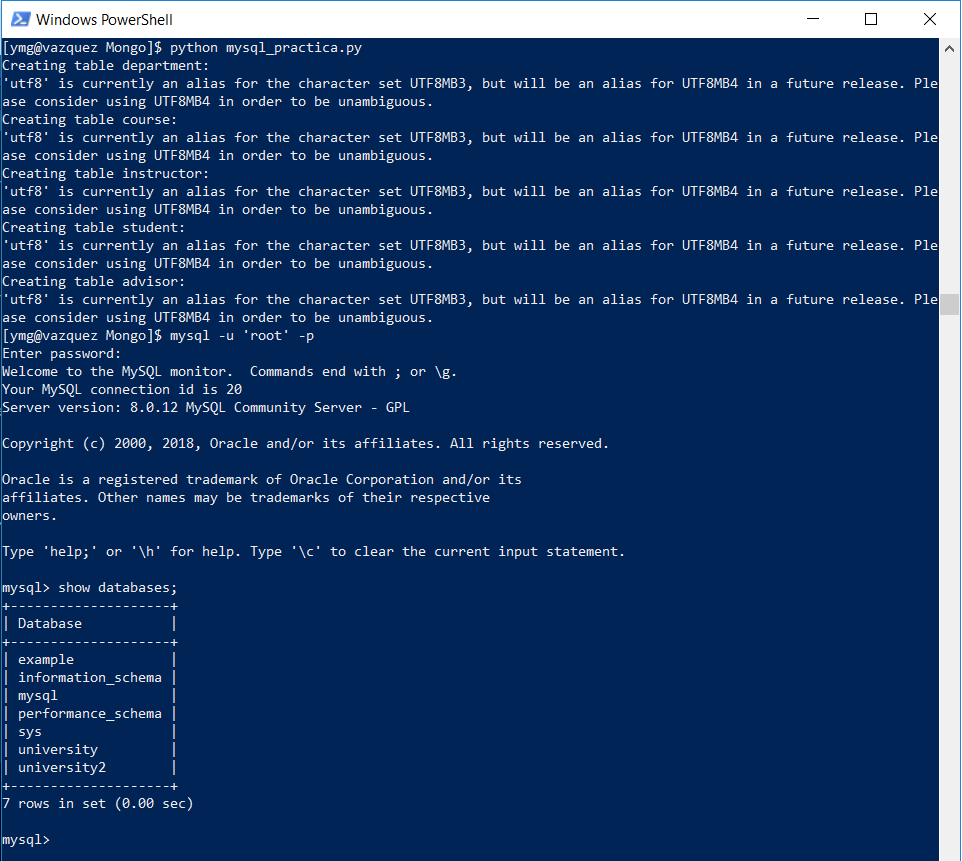
\includegraphics{ejec.png}
\end{figure}

Chequeo de tablas y contenido:

\begin{figure}[htbp]
\centering
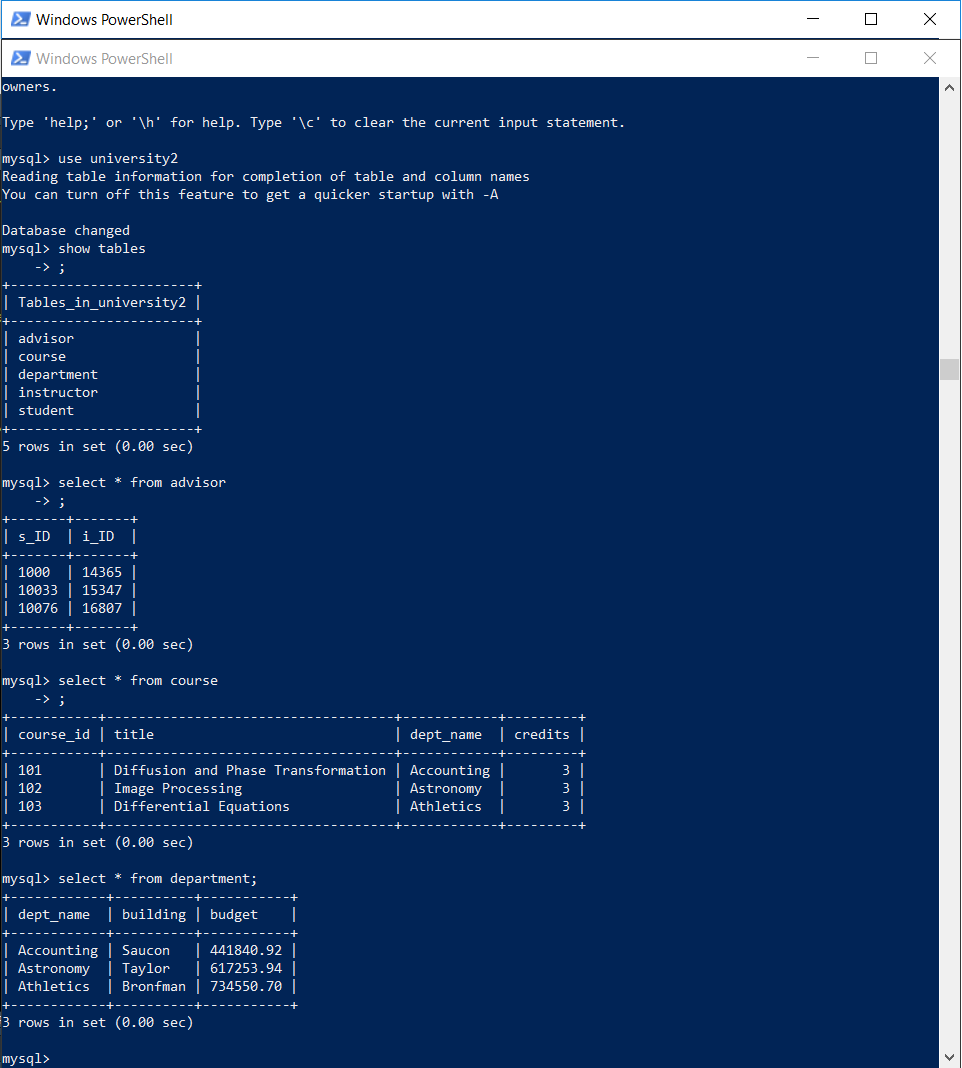
\includegraphics{tablas1.png}
\end{figure}

\begin{figure}[htbp]
\centering
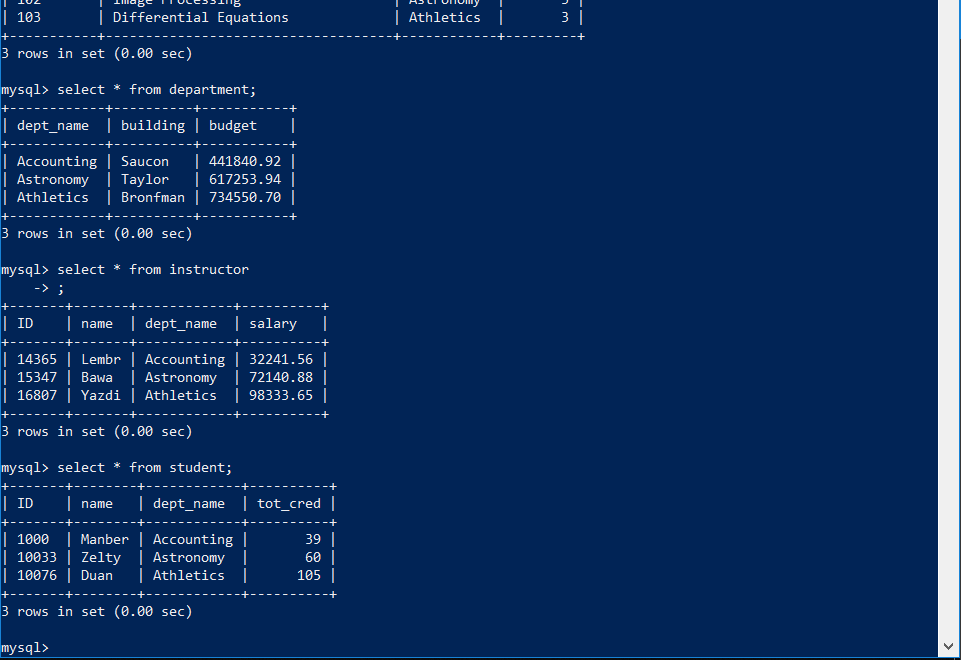
\includegraphics{tablas2.png}
\end{figure}


\end{document}
